\section{Prozessplanung}
\label{sec:prozessplanung}

Wie beschrieben, ist der erste Schritt, eine Frontendapplikation zu entwickeln, welche einer Liste von Ansprüchen genügt. Hauptaspekt dieser Software soll die feingranulare Planung von Fertigungsprozessen sein.\\
Im folgenden Kapitel werden zunächst die erforderlichen Kriterien herausgearbeitet und diskutiert und auch mögliche Schwachstellen untersucht, während sich das darauffolgende Kapitel mit der Implementierung befasst. Kapitel \ref{sec:prozesssteuerung} baut dann weiter auf den hier erarbeiteten Konzepten auf und erweitert diese. Die hier als „Prozessplanung“ beschriebene Applikation versteht sich also als ein reines Frontend-Programm.

\subsection*{Konzeption}
\label{subsec:prozessplanung_konzeption}

Um die Ansprüche nun näher zu definieren, ist es zunächst erforderlich, die Zielgruppe dieser Applikation zu identifizieren. Trotz dieses konkreten Anwendungsfalls – als Teil der Digital Twin Platform – soll aber nicht der Aspekt der Potenzialanalyse dieser Arbeit vernachlässigt werden. Daher ist es nötig, dass die Zielgruppe nicht ausschließlich durch die Gruppe der Benutzer dieser Webseite eingegrenzt wird, sondern dass auch eine allgemeinere Zielgruppe in Betracht gezogen wird. Diese Gruppe reicht von unerfahrenen Laien, welche etwa die Digital Twin Academy Webseite nutzen, um erste Erfahrungen mit IIoT und der Planung von Prozessabläufen zu sammeln, bis hin zu erfahrenem Personal, welches das Prozessplanungs-Interface nutzt, um komplexe Prozesse an einer vertrauten Anlage zu planen. Letztere Teilgruppe hat evidenterweise bereits Werkzeuge für die Prozessplanung, doch diese sind in der Regel nicht einfach von der ersteren Teilgruppe nutzbar oder es fehlt an IIoT Fähigkeiten.\\
Das zu entwickelnde Programm sollte also für Laien einfach benutzbar sein, aber dennoch Experten nicht einschränken, sondern ihnen Funktionen zur Hand geben, um ihre Arbeit mit dem Programm zu erleichtern und zu beschleunigen. Außerdem sollte das Programm leicht zu lernen und intuitiv sein; es soll gewährleistet werden, dass Nutzer sich nicht erst in komplexe Dokumentationen einlesen müssen, sondern nach dem „learning by doing“ Prinzip agieren können.\\
Zusammenfassend lassen sich also folgende aus der Zielgruppe abgeleitete Kriterien für die angestrebte Softwarelösung festhalten:

\begin{enumerate}
    \item \textbf{Simplizität} – Die Benutzeroberfläche soll leicht zu benutzen sein, auch für Benutzer, welche nicht oder kaum mit dem Anwendungsraum vertraut sind
    \item \textbf{Vielschichtigkeit} – Die Simplizität soll Expertennutzer nicht einschränken, sondern es soll Funktionalitäten geben, welche die Benutzung für diese Gruppe beschleunigt
    \item \textbf{Intuitivität} – Die Lernkurve soll möglichst flach sein, sodass ein Nutzer sich nicht erst einlesen muss
\end{enumerate}

Als Nächstes ist es relevant, die Platform zu identifizieren. Auch unabhängig von der konkreten Implementierungsplatform (Digital Twin Platform) sollte ein allgemein zugängliches Programm möglichst einfach zu initialisieren sein. Bei Weitem am simpelsten ist hier offensichtlich ein Web-Interface, da damit – abgesehen von einem Web-Browser welcher ohnehin vorinstalliert ist – keine Software installiert werden muss. Um eine hohe Kompatibilität zu gewährleisten, muss sichergestellt werden, dass das Programm in einem möglichst hohen Anteil an Web-Browser funktioniert und von möglichst vielen potenziellen Nutzern benutzbar ist.\\
Als eine Richtlinie soll der „Europa Web Guide“ [\cite{guidelineWeb}] genutzt werden, welcher ein Regelbuch für die Webpräsenz der Europäischen Kommission darstellt. Da diese Richtlinien jedoch speziell für die Internetpräsenz der Europäischen Kommission angefertigt wurden, müssen einige Punkte für diesen Anwendungsfall abgeändert werden, wobei es dennoch eine nützliche Richtlinie bleibt.\nocite{guidelineBrowserSupport}\nocite{guidelineDataProtextion}

Da keine konkreten Nutzeranalysedaten für die Webseite der Digital Twin Academy vorliegen, ist das Ziel also eine Abdeckung aller Desktop-Browser, welche einen Marktanteil von 3 \% oder mehr haben. Wie in Grafik \ref{fig:Browser_Market_Share} zu sehen ist, betrifft dies mit Stand vom Dezember 2021 die fünf Browser Chrome, Safari, Edge, Firefox und Opera [\cite{browserMarketShare}].
%
\begin{figure}[htbp]
	\centering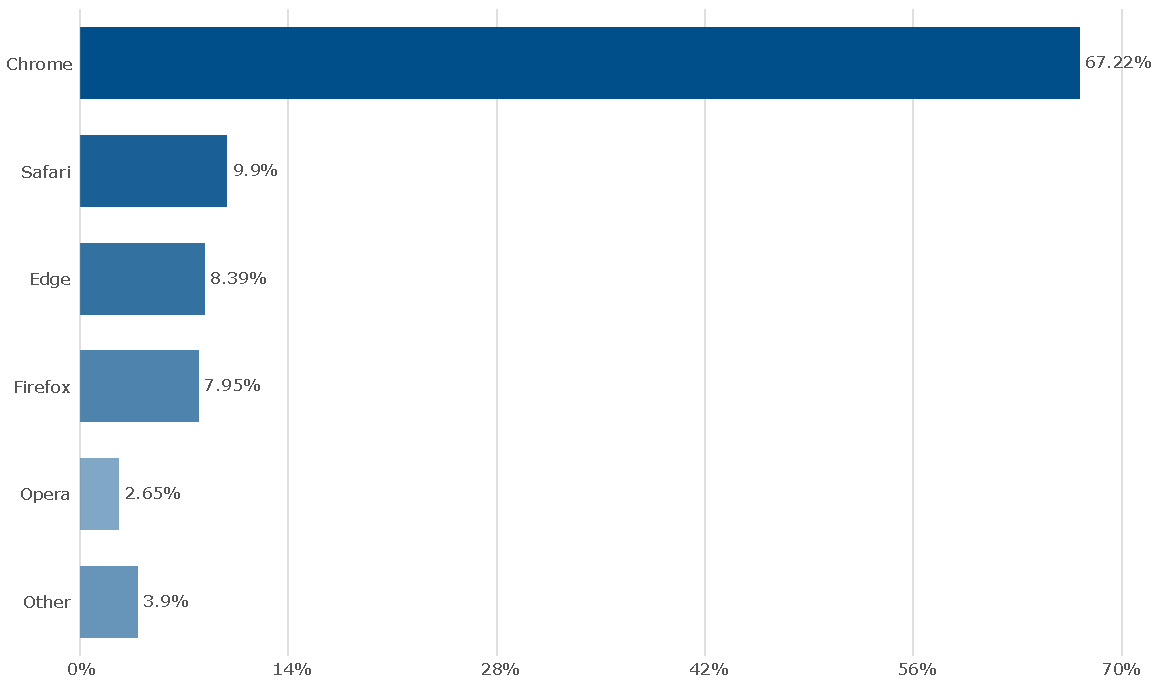
\includegraphics[width=1.0\textwidth]{images/04/Browser_Stats.pdf}
    \caption{Desktop-Browser-Marktanteil weltweit [\cite{browserMarketShare}]}
    \label{fig:Browser_Market_Share}
\end{figure}

Die Browserversionen betreffend sollten alle Versionen der letzten zwölf Monate unterstützt werden. Diese Zahl ist grob basierend auf der Annahme von neuen Browserversionen, da in der Regel über 98 \% der Nutzer eine Version benutzen, welche jünger als zwölf Monate alt ist [\cite{browserVersionAdoption}].\\
Zum Stand vom Dezember 2021 ergeben sich also die in Tabelle \ref{tab:browserMinVersionen} zu unterstützenden Versionen.
%
\bgroup
\def\arraystretch{1.5}
\vspace{5mm}\begin{table}[htbp]
    \centering
    \begin{tabularx}{100mm}{@{}p{60mm}|*1{>{\centering\arraybackslash}X}@{}}
        \rowcolor{dikblue} \mbox{\color{white}\textbf{Browser}} & \mbox{\color{white}\textbf{Versionen}} \\
        Google Chrome   & 88 – 97 \\ \hline
        Apple Safari    & 14 – 15 \\ \hline
        Microsoft Edge  & 88 – 96 \\ \hline
        Mozilla Firefox & 78 – 95 \\ \hline
        Opera           & 74 – 76 \\ \hline
    \end{tabularx}
    \caption{Zu unterstützende Browser-Versionen}
    \label{tab:browserMinVersionen}
\end{table}
\egroup

Aus dem Kriterium, dass der Browser als Platform dienen sollte, kann zudem abgeleitet werden, dass das Programm in JavaScript geschrieben werden soll; konkreter in ECMAScript 2020 (ES11). Über Kompatibilitätsschichten sind theoretisch auch andere Sprachen denkbar, allerdings ist ECMAScript 2020 die einzige (Frontend-)Programmiersprache, welche von den allen aktuellen Browsern unterstützt wird. Die einzige Ausnahme hierzu bildet das relativ neue WebAssembly (WASM), doch WASM wäre für eine solche Frontendapplikation exzessiv.

Aus den Erkenntnissen über die Platform lassen sich also folgende weitere Kriterien gewinnen:

\begin{enumerate}
    \setcounter{enumi}{3}
    \item \textbf{Zugängliche Platform} – Das Programm soll im Web-Browser laufen, sodass es nicht installiert werden muss und (praktisch) sofort benutzt werden kann
    \item \textbf{JavaScript} – Als Programmiersprache soll ECMAScript 2020 genutzt werden
    \item \textbf{Touchoptimiert} – Das Interface sollte auch auf größeren Touch-Geräten wie Tablets oder Laptops mit Touch-Funktion benutzbar sein
\end{enumerate}

Außerdem lassen sich weitere Kriterien aus der Design-Prinzipien von Industrie 4.0 (siehe Kapitel \ref{subsec:industrie40design}) ziehen:

\begin{enumerate}
    \setcounter{enumi}{6}
    \item \textbf{Dezentralisierung} – Es sollen Prozessabläufe für Anlagen an beliebigen Standorten geplant werden können
    \item \textbf{Virtualisierung} – Die geplanten Prozesse sollen virtualisierbar sein
    \item \textbf{Interoperabilität} – Es soll vom Hersteller abstrahiert werden, sodass Anlagen von beliebigen Herstellern planbar sind
    \item \textbf{Serviceorientierung} – Die Applikation soll als Service aufgebaut werden, um sie in Zukunft gegen einen anderen Service austauschen zu können
    \item \textbf{Modularität} – Das Gesamtkonstrukt soll in Module eingegliedert werden, sodass es nach Belieben an veränderte Ansprüche angepasst werden kann
    \item \textbf{Echtzeitfähigkeit} – Es sollen Prozesse geplant werden können, welche vom aktuellen Zustand der Anlage abhängig sind; außerdem sollen Latenzen und Latenz-Varianzen (engl.: Jitter) in einem für Echtzeitsysteme akzeptablen Rahmen bleiben
\end{enumerate}
